\documentclass[10pt,a4paper]{article}

\usepackage[T1]{fontenc}
\usepackage[utf8]{inputenc}
\usepackage{lmodern}
\usepackage{microtype}
\usepackage[a4paper,left=18mm,right=18mm,top=25mm,bottom=20mm,headheight=17mm,headsep=8mm,footskip=10mm]{geometry}
\usepackage{xcolor}
\usepackage{graphicx}
\usepackage{tabularx}
\usepackage{array}
\usepackage{booktabs}
\usepackage{enumitem}
\usepackage{titlesec}
\usepackage{tcolorbox}
\usepackage{fancyhdr}
\usepackage{lastpage}
\usepackage{tikz}
\usepackage{hyperref}
\hypersetup{hidelinks}
\usepackage[backend=biber,style=ieee,sorting=none]{biblatex}
\addbibresource{../ref.bib}

% -----------------------------------------------------------------------------
% Colours sampled/approximated from the original document
% -----------------------------------------------------------------------------
\definecolor{MetroBlue}{HTML}{23477F}
\definecolor{MetroOrange}{HTML}{F39200}
\definecolor{BodyText}{HTML}{202B3A}
\definecolor{Muted}{HTML}{65748A}
\definecolor{RuleGray}{HTML}{D3D6DA}
\definecolor{PanelGray}{HTML}{F1F2F4}
\definecolor{ConfRed}{HTML}{C9252B}

\color{BodyText}
\setlength{\parindent}{0pt}
\setlength{\parskip}{0pt}
\renewcommand{\familydefault}{\sfdefault}

% -----------------------------------------------------------------------------
% Header and footer
% -----------------------------------------------------------------------------
\newcommand{\ConfidentialBox}{%
  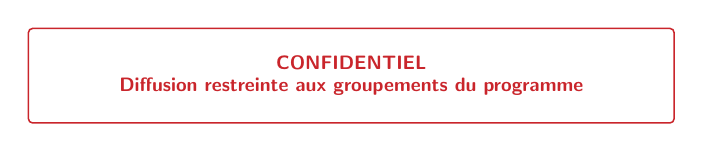
\begin{tikzpicture}[baseline=(current bounding box.center)]
    \node[draw=ConfRed, rounded corners=1.5pt, line width=.55pt,
      minimum width=82mm, minimum height=12mm, align=center,
      text=ConfRed, font=\bfseries\fontsize{6.7}{8}\selectfont, inner sep=2pt]
      {CONFIDENTIEL\\Diffusion restreinte aux groupements du programme};
  \end{tikzpicture}%
}
\pagestyle{fancy}
\fancyhf{}
\fancyhead[L]{\raisebox{1.5mm}{\color{Muted}\fontsize{7.2}{8.5}\selectfont
  Metropolis $\cdot$ Programme Renouvellement Signalisation $\cdot$ GTS}}
\fancyhead[R]{\ConfidentialBox}
\fancyfoot[R]{\color{Muted}\fontsize{7.5}{9}\selectfont\thepage\,/\,4}
\renewcommand{\headrulewidth}{0pt}
\renewcommand{\footrulewidth}{0pt}

% -----------------------------------------------------------------------------
% Section heading style
% -----------------------------------------------------------------------------
\titleformat{\section}
  {\normalfont\bfseries\Large\color{MetroBlue}}
  {\textcolor{MetroOrange}{\thesection.}}{0.55em}{}
\titlespacing*{\section}{0pt}{0pt}{8pt}

% Action/expectation procedure panels
\newtcolorbox{procedurebox}{
  colback=PanelGray,
  colframe=PanelGray,
  boxrule=.45pt,
  arc=2mm,
  left=4mm,right=4mm,top=2.5mm,bottom=2.5mm,
  before skip=8pt, after skip=0pt
}

\newlist{teststeps}{enumerate}{1}
\setlist[teststeps]{label=\arabic*., leftmargin=6mm, labelsep=2mm,
  itemsep=3.3pt, topsep=3pt, parsep=0pt, partopsep=0pt}
\newlist{substeps}{enumerate}{1}
\setlist[substeps]{label=\alph*., leftmargin=7mm, labelsep=2mm,
  itemsep=3pt, topsep=3pt, parsep=0pt, partopsep=0pt}

\begin{document}

% =============================================================================
% PAGE 1 — COVER / DOCUMENT INFORMATION
% =============================================================================
\thispagestyle{fancy}

\vspace*{1mm}
\noindent
\begin{minipage}[c]{0.59\textwidth}
  
\includegraphics[height=1.4cm,keepaspectratio]{../logo/LogoMetropolis.pdf}
\end{minipage}%
\begin{minipage}[c]{0.40\textwidth}
  \raggedleft
  
\includegraphics[height=0.45cm,keepaspectratio]{../logo/LogoProver.pdf}
\end{minipage}

\vspace{12mm}
{\color{MetroOrange}\bfseries\fontsize{8.2}{10}\selectfont
  P R O G R A M M E\quad R E N O U V E L L E M E N T\quad S I G N A L I S A T I O N\par}

\vspace{4mm}
{\color{MetroBlue}\bfseries\fontsize{25}{30}\selectfont
  Generic Test Specification for\\[-1mm]
  Metropolis GA package\par}

\vspace{2mm}
{\color{Muted}\fontsize{10.5}{13}\selectfont Version 2.0, 2026-11-06\par}

\vspace{10mm}
{\color{Muted}\bfseries\fontsize{7.5}{9}\selectfont REVISION HISTORY\par}
\vspace{2mm}
\renewcommand{\arraystretch}{1.55}
\begin{tabularx}{\textwidth}{@{}>{\raggedright\arraybackslash}p{0.13\textwidth}
  >{\raggedright\arraybackslash}p{0.17\textwidth}
  >{\raggedright\arraybackslash}p{0.13\textwidth}
  >{\raggedright\arraybackslash}X@{}}
  \textcolor{Muted}{\bfseries\fontsize{7}{8}\selectfont VERSION} &
  \textcolor{Muted}{\bfseries\fontsize{7}{8}\selectfont DATE} &
  \textcolor{Muted}{\bfseries\fontsize{7}{8}\selectfont AUTHOR} &
  \textcolor{Muted}{\bfseries\fontsize{7}{8}\selectfont CHANGE} \\
  \midrule
  0.1 & 2022-06-15 & DF & Draft version for review \\
  \midrule
  1.0 & 2022-11-04 & GZ & This document is aligned with the formal GTS \\
  \midrule
  2.0 & 2026-11-06 & G & This document is aligned with the formal GTS \\
  \bottomrule
\end{tabularx}

\vspace{4mm}
\begin{tcolorbox}[
  colback=PanelGray,colframe=PanelGray,boxrule=0pt,arc=2mm,
  left=4mm,right=4mm,top=3mm,bottom=2.5mm]
  {\color{Muted}\bfseries\fontsize{7.5}{9}\selectfont CONTENTS\par}
  \vspace{2mm}
  \begin{enumerate}[label=\textcolor{MetroOrange}{\bfseries\arabic*.},
    leftmargin=5mm,labelsep=2mm,itemsep=2.5mm,topsep=0pt,parsep=0pt]
    \item Introduction
    \item Initialization
    \item Test Case 1
    \item Test Case 2 — Manual switch throwing
    \item Test Case 3 — Line block interface for exit signals
    \item Test Case 4 — Manual release
  \end{enumerate}
\end{tcolorbox}

\newpage

% =============================================================================
% PAGE 2 — TEST SPECIFICATION
% =============================================================================
\section{Introduction}
This is the informal Generic Test Specification for the Metropolis GA package.

\vspace{9mm}
\section{Initialization}
The purpose of this test, or rather procedure, is to set up the system in such a way that the test cases can be performed.

\begin{procedurebox}
  \begin{teststeps}
    \item \textnormal{[Action]} Set all tracks clear.
    \item \textnormal{[Action]} Set the line input of every exit signal.
  \end{teststeps}
\end{procedurebox}

\vspace{9mm}
\section{Test Case 1}
The purpose of this test is to test all the major functionalities.

\begin{procedurebox}
  \textbf{For each route:}
  \begin{teststeps}
    \item \textnormal{[Action]} Initialize the system.
    \item \textnormal{[Action]} Request every switch in the route in its proper position.
    \item \textnormal{[Action]} Request a sufficient set of protective switches (which might be empty) in their protective positions.
    \item \textnormal{[Expect]} All switches in the route are in proper correspondence.
    \item \textnormal{[Expect]} The flank of the route is protected.
    \item \textnormal{[Expect]} If the route does not end in a buffer stop or an exit signal, the front of the route is protected.
    \item \textnormal{[Action]} Request the route.
    \item \textnormal{[Expect]} The route is set.
    \item \textnormal{[Expect]} The start signal is commanded to proceed and shows proceed.
    \item \textnormal{[Action]} Occupy the track immediately before the route.
    \item \textnormal{[Action]} Occupy the first track of the route.
    \item \textnormal{[Expect]} The start signal is neither commanded to proceed nor shows proceed.
    \item \textnormal{[Action]} Vacate the track immediately before the route.
    \item Traverse the rest of the route and assert that locking of route sections releases as the train passes over them.
      For each track tc in the route (except for the first track):
      \begin{substeps}
        \item \textnormal{[Action]} Occupy tc.
        \item \textnormal{[Action]} Vacate the track before tc.
        \item \textnormal{[Expect]} If the track just vacated is the last track in the route section that contains it, the locking of this route section is released.
      \end{substeps}
    \item \textnormal{[Action]} Occupy the track immediately after the route.
    \item \textnormal{[Action]} Vacate the last track of the route.
    \item \textnormal{[Expect]} The locking of the last route section is released.
  \end{teststeps}
\end{procedurebox}

\vspace{9mm}
\section{Test Case 2}
The purpose of this test is to test manual switch throwing and to verify that a switch cannot be moved when its track circuit is occupied.

\begin{procedurebox}
  \textbf{For each switch:}
  \begin{teststeps}
    \item \textnormal{[Action]} Request the switch to reverse position.
    \item \textnormal{[Expect]} The switch loses normal detection within 1s.
    \item \textnormal{[Expect]} The switch gains reverse detection within 4s.
    \item \textnormal{[Action]} Request the switch to normal position.
    \item \textnormal{[Expect]} The switch loses reverse detection within 1s.
    \item \textnormal{[Expect]} The switch gains normal detection within 4s.
    \item \textnormal{[Action]} Occupy the track circuit that contains the switch.
    \item \textnormal{[Action]} Request the switch to reverse position.
    \item \textnormal{[Expect]} The switch stays in normal position during 60s.
  \end{teststeps}
\end{procedurebox}

\vspace{9mm}
\section{Test Case 3}
The purpose of this test is to test the line block interface for routes that end in an exit signal.

\begin{procedurebox}
  \textbf{For each route that ends in an exit signal:}
  \begin{teststeps}
    \item \textnormal{[Action]} Initialize the system.
    \item \textnormal{[Action]} Request every switch in the route in its proper position.
    \item \textnormal{[Action]} Request a sufficient set of protective switches (which might be empty) in their protective positions.
    \item \textnormal{[Expect]} All switches in the route are in proper correspondence.
    \item \textnormal{[Expect]} The flank of the route is protected.
    \item \textnormal{[Action]} Set the line input of the exit signal to false.
    \item \textnormal{[Expect]} The line output of the exit signal is true during 5s.
    \item \textnormal{[Action]} Request the route.
    \item \textnormal{[Expect]} No section of the route becomes locked during 30s.
    \item \textnormal{[Action]} Set the line input of the exit signal to true.
    \item \textnormal{[Action]} Request the route.
    \item \textnormal{[Expect]} The route becomes locked within 5s.
    \item \textnormal{[Expect]} The start signal of the route shows proceed within 1s.
    \item \textnormal{[Expect]} The line output of the exit signal is false during 5s.
    \item \textnormal{[Action]} Request manual release of the route.
    \item \textnormal{[Expect]} All route sections of the route are unlocked.
    
  \end{teststeps}
\end{procedurebox}

\vspace{9mm}
\section{Test Case 4}
The purpose of this test is to test that a manual release request removes the proceed command at once and releases all route sections simultaneously after the 30s delay.

\begin{procedurebox}
  \textbf{For each route:}
  \begin{teststeps}
    \item \textnormal{[Action]} Initialize the system.
    \item \textnormal{[Action]} Request every switch in the route in its proper position.
    \item \textnormal{[Action]} Request a sufficient set of protective switches (which might be empty) in their protective positions.
    \item \textnormal{[Action]} If the route ends in an exit signal, set the line input of the exit signal to true.
    \item \textnormal{[Expect]} All switches in the route are in proper correspondence.
    \item \textnormal{[Expect]} The flank of the route is protected.
    \item \textnormal{[Expect]} If the route does not end in a buffer stop or an exit signal, the front of the route is protected.
    \item \textnormal{[Action]} Request the route.
    \item \textnormal{[Expect]} The route is set.
    \item \textnormal{[Expect]} The start signal is commanded to proceed and shows proceed.
    \item \textnormal{[Action]} Request release of the route.
    \item \textnormal{[Expect]} The start signal is neither commanded to proceed nor shows proceed.
    \item \textnormal{[Expect]} The route is not set.
    \item \textnormal{[Expect]} During the following 28s, all route sections stay locked and the start signal is not commanded to proceed.
    \item \textnormal{[Expect]} During the following 4s, the route sections are either all locked or all unlocked at every instant, i.e. they release simultaneously.
    \item \textnormal{[Expect]} All route sections of the route are unlocked.
  \end{teststeps}
\end{procedurebox}

\end{document}